%++++++++++++++++++++++++++++++++++++++++
% Don't modify this section unless you know what you're doing!
\PassOptionsToPackage{table}{xcolor}
\PassOptionsToPackage{xcdraw}{xcolor}

\documentclass[letterpaper,10pt]{article}
\usepackage{tabularx} % extra features for tabular environment
\usepackage{amsmath}  % improve math presentation
\usepackage{graphicx} % takes care of graphic including machinery
\usepackage[margin=1in,letterpaper]{geometry} % decreases margins
\usepackage{cite} % takes care of citations
\usepackage[final]{hyperref} % adds hyper links inside the generated pdf file
 \usepackage[table,xcdraw]{xcolor}
\usepackage{eurosym}
\usepackage{fontawesome}
\usepackage{float}
\usepackage{wrapfig,booktabs}
\usepackage{hyperref}

\definecolor{gutsgreen}{RGB}{0, 211, 160}
\definecolor{gutsoranje}{RGB}{255, 106, 76}

% \usepackage{titling}
% \setlength{\droptitle}{-3cm}

\hypersetup{
	colorlinks=true,       % false: boxed links; true: colored links
	linkcolor=blue,        % color of internal links
	citecolor=blue,        % color of links to bibliography
	filecolor=magenta,     % color of file links
	urlcolor=blue         
}
%++++++++++++++++++++++++++++++++++++++++
\usepackage{subcaption}

% \usepackage[showframe=true]{geometry}
\usepackage{geometry}
% \usepackage{changepage}
\usepackage{subcaption}
\pagenumbering{gobble}

\geometry{
a4paper,
total={170mm,257mm},
left=10mm,
right=10mm,
top=10mm,
bottom=10mm
}
 
\begin{document}

\title{ %
\vspace{-2cm}

\includegraphics{1} \\
Guaranteed Entrance Token \\
\small Summary of the GET-Protocol}
\date{}

\maketitle
\vspace{-1.5cm}
% \begin{table}[H]
% \centering
% \label{my-label}
% \begin{tabular}{|
% >{\columncolor[HTML]{FFFFFF}}l |
% >{\columncolor[HTML]{FFFFFF}}l |
% >{\columncolor[HTML]{FFFFFF}}l |}
% \hline
% 1 October - 15 Oktober ('17) & 5 pricing tiers                                                                                       & 4 rounds per tier                                                                                         \\ \hline
% Min Cap: \euro 2.5 million   & \begin{tabular}[c]{@{}l@{}}Tokens will be immediately distributed\\  after the ICO ends.\end{tabular} & \begin{tabular}[c]{@{}l@{}}If cap not reached; full refund to \\ investors (minus gas costs)\end{tabular} \\ \hline
% Max Cap: \euro 15.2 million  & In total 90 million tokens will be issued.                                                            & Accepted currencies: ETH, BTC, ETC                                                                        \\ \hline
% \end{tabular}
% \caption{Summary of the GET ICO.}
% \end{table}

\begin{center}
\textit{The GET Protocol is a blockchain-based protocol that is used by ticketing companies to completely merge the primary and secondary ticketing market. The protocol gives complete control over the sale and trade between ticket holder from the moment the first ticket is sold until the last ticket is scanned. The platform's own ERC20 token, the GET, functions as a FIAT value locking asset in a user's wallet/smart ticket. The FIAT value of GET is set at the start of an event cycle. By this value locking mechanism all actors are shielded from crypto volatility during an event cycle. GUTS Tickets is based in Amsterdam, The Netherlands, and has a working smart ticketing application that is already used by big event organizers in the Netherlands. This experience and operational readiness of its team makes the company perfectly positioned to develop the GET Protocol as the company is able to build the protocol and improve and deploy it incrementally.}
\end{center}

\subsection*{GUTS Tickets, The GET Foundation \& the future of ticketing}
\begin{wraptable}[17]{r}{11cm}
\centering
% \caption{My caption}
% \label{my-label}
\begin{tabular}{cc}
\rowcolor[HTML]{000000} 
{\color[HTML]{FFFFFF} \textbf{GUTS Tickets}}                                                                                                      & {\color[HTML]{FFFFFF} \textbf{The GET Foundation}}                                                                                                       \\
\multicolumn{1}{|c|}{Provides smart ticketing services}                                                                                           & \multicolumn{1}{c|}{Provides a open blockchain protocol}                                                                                                 \\
\rowcolor[HTML]{C0C0C0} 
\multicolumn{1}{|l|}{\cellcolor[HTML]{C0C0C0}\begin{tabular}[c]{@{}l@{}}\textbf{Customers:} Event organizers, \\ festivals and venue owners.\end{tabular}} & \multicolumn{1}{l|}{\cellcolor[HTML]{C0C0C0}\begin{tabular}[c]{@{}l@{}}\textbf{Customers:} Ticketing companies, \\ promotors and booking companies.\end{tabular}} \\
\multicolumn{1}{|c|}{\begin{tabular}[c]{@{}c@{}}Builds consumer facing smart\\ ticketing web-application.\end{tabular}}                           & \multicolumn{1}{c|}{\begin{tabular}[c]{@{}c@{}}Provides a value conserving\\ protocol for ticketing companies.\end{tabular}}                             \\
\rowcolor[HTML]{C0C0C0} 
\multicolumn{1}{|c|}{\cellcolor[HTML]{C0C0C0}Operational since Q1 2016}                                                                           & \multicolumn{1}{c|}{\cellcolor[HTML]{C0C0C0}White paper published Q2 2017}                                                                               \\
\multicolumn{1}{|c|}{\begin{tabular}[c]{@{}c@{}}Launching customer: Hekwerk\\ 310.000 ticket / year.\end{tabular}}                                & \multicolumn{1}{c|}{\begin{tabular}[c]{@{}c@{}}Launching customer: \\ GUTS Tickets\end{tabular}}                                                         \\
\rowcolor[HTML]{C0C0C0} 
\multicolumn{1}{|c|}{\cellcolor[HTML]{C0C0C0}\begin{tabular}[c]{@{}c@{}}GUTS Tickets BV\\ Registrant number: 69771138\end{tabular}}               & \multicolumn{1}{c|}{\cellcolor[HTML]{C0C0C0}\begin{tabular}[c]{@{}c@{}}GET Foundation (Stichting)\\ Registrant number: 65911296\end{tabular}}            \\ \hline
\multicolumn{2}{|c|}{\begin{tabular}[c]{@{}c@{}}Both entities are incorporated in the Netherlands and\\ are fully compliant with Dutch/EU rules and regulations.\end{tabular}}                                                                                                                               \\ \hline
\end{tabular}
% \vspace{-10pt}
\caption{ \textbf{The difference between GUTS Tickets and the GET Foundation. } }
\end{wraptable}

The ticketing company \textbf{GUTS} is currently selling blockchain-registered tickets via its smart-ticketing application. In 2017 alone the company sold tickets for more than 30 events totaling more than 10.000 tickets. Where traditional ticketing companies provide a buyer with a static QR code, the GUTS application serves the user with a dynamic QR code that changes as a function over time and owner. One of the Netherlands most prominent theater companies, \href{https://hekwerk.nl/}{\textcolor{gutsoranje}{Hekwerk Theaterproducties}}, have partnered with GUTS and its team. \href{https://blog.guts.tickets/the-hekwerk-deal-7554071b26c1}{\textcolor{gutsoranje}{This deal alone}} secures protocol usage for more than 310.000 tickets in 2019. Several prominent artists and their management, one of which is \href{https://blog.guts.tickets/advisory-board-of-get-watse-de-jong-manager-martin-garrix-nyle-budimlic-cypher-group-32ec30ce06ae}{\textcolor{gutsoranje}{Martin Garrix}}, have shown their support for our vision of a efficient and transparent primary and secondary ticketing market, cutting out the profits made by parties adding little to no value in the value chain. The protocol allows ticket owners to resell their ticket anonymously to other consumers directly in the web-app without the risk of being defrauded or getting  scalping with fees/excessive margins. 

\textbf{We are live.} The GET Protocol is more than a white paper or a proof of concept. It is reality. GUTS Tickets is already selling smart tickets registered on the blockchain. After the crowdsale is completed other functionalities as reselling tickets within a price margin will be added to the protocols functionality. Check out the \href{https://events.guts.tickets/events}{\textcolor{gutsoranje}{events}} we ticket for or try out the \href{https://sandbox.guts.tickets/events/8}{\textcolor{gutsoranje}{sandbox}} environment and experience the future of ticketing for yourself.

% \textcolor{gutsoranje}{events}

%  \vspace{-3cm}
\begin{table}[h]
\centering
%\caption{My caption}
\resizebox{\textwidth}{!}{%
\begin{tabular}{|l|c|c|c|}
\hline
\rowcolor[HTML]{000000} 
\multicolumn{1}{|c|}{\cellcolor[HTML]{000000}{\color[HTML]{FFFFFF} \textbf{GET Protocol}}} & {\color[HTML]{FFFFFF} \textbf{\euro Euro}}                                 & {\color[HTML]{FFFFFF} \textbf{Status}}                                                                                       & {\color[HTML]{FFFFFF} \textbf{Total GET}}      \\ \hline
\rowcolor[HTML]{C0C0C0} 
\textbf{Softcap}                                                                           & \euro 2.3 million                                                          & \textbf{\begin{tabular}[c]{@{}c@{}}Reached \\ After completing public pre-sale\end{tabular}}                                 & 8.560.800 GET                                  \\ \cline{1-1}
\rowcolor[HTML]{FFFFFF} 
\textbf{Hardcap goal}                                                                      & \euro15 million                                                            & \begin{tabular}[c]{@{}c@{}}Crowdsale is completed\\ (ended 13 December 13 CET)\end{tabular}                                  & 23.987.367 GET                                 \\ \cline{1-1}
\rowcolor[HTML]{C0C0C0} 
\textbf{Crowdsale result}                                                                  & \euro 6.253.185 million                                                    & 10.934,62 ETH                                                                                                                & 9.901.391,97 GET                               \\ \cline{1-1}
\rowcolor[HTML]{FFFFFF} 
\textbf{Circulating supply}                                                                & \multicolumn{2}{c|}{\cellcolor[HTML]{FFFFFF}Crowdsale + Bounty Referral partitions}                                                                                                                       & 10.384.386,70 GET                              \\ \cline{1-1}
\rowcolor[HTML]{C0C0C0} 
\textbf{Maximum supply}                                                                    & \multicolumn{2}{c|}{\cellcolor[HTML]{C0C0C0}\begin{tabular}[c]{@{}c@{}}Meaning all GET to be ever minted. There will be never more GET than \\ this amount of GET in existence.\end{tabular}}             & 33.368.773,40 GET*                             \\ \hline
\textbf{Total burned}                                                                      & \multicolumn{3}{l|}{\begin{tabular}[c]{@{}l@{}}In total two token burns where conducted. One at the half-way point and the last one at finalization.\\ of the crowdsale. Both burn summed amount to a total of: 56.631.226,60 GET burned.\end{tabular}}    \\ \hline
\rowcolor[HTML]{C0C0C0} 
\textbf{\begin{tabular}[c]{@{}l@{}}Average GET price\\ during complete sale\end{tabular}}  & \multicolumn{3}{l|}{\cellcolor[HTML]{C0C0C0}\begin{tabular}[c]{@{}l@{}}On average (including the private \& public pre-sale) contributors received 0.00110435179 GET/ETH.\\ In total 1179 unique contributors participated in the crowdsale.\end{tabular}} \\ \hline
\end{tabular}%
}
\caption{Summary of the GET Protocol ICO. \href{https://blog.guts.tickets/feel-the-burn-6f0315c6721e}{\textcolor{gutsoranje}{ Details about the recalibration of the hardcap on the half-way point due to the increased ether price is described in our blog.}}}
\end{table}
% Please add the following required packages to your document preamble:
% \usepackage[table,xcdraw]{xcolor}
% If you use beamer only pass "xcolor=table" option, i.e. \documentclass[xcolor=table]{beamer}
% \begin{table}[h]
% \centering

% \label{my-label}
% \begin{tabular}{|l|c|c|c|}
% \hline
% \rowcolor[HTML]{000000} 
% \multicolumn{1}{|c|}{\cellcolor[HTML]{000000}{\color[HTML]{FFFFFF} \textbf{GUTS/GET-protocol}}} & {\color[HTML]{FFFFFF} \textbf{Euro}} & {\color[HTML]{FFFFFF} \textbf{Ether Lockprice*}} & {\color[HTML]{FFFFFF} \textbf{Total GET}} \\ \hline
% \rowcolor[HTML]{C0C0C0} 
% \textbf{Softcap*} & \euro2.3 million & Reached & 8.560.800 GET \\ \cline{1-1}
% \rowcolor[HTML]{FFFFFF} 
% \textbf{Hardcap} & \euro15 million & \begin{tabular}[c]{@{}c@{}}Crowdsale will end\\ on 13/12/17 13:00 CET.\end{tabular} & 90.000.000 GET \\ \cline{1-1}
% \rowcolor[HTML]{C0C0C0} 
% \textbf{Pre-sale private*} & \euro 1.8 million & \euro 258.29/ETH & 7.200.000 GET \\ \cline{1-1}
% \rowcolor[HTML]{FFFFFF} 
% \textbf{Pre-sale public*} & \euro 0.5 million & \euro 262.17/ETH & 1.351.351 GET \\ \cline{1-1}
% \rowcolor[HTML]{C0C0C0} 
% \textbf{General sale} & \euro 12.7 million & \euro 275.44/ETH & 15,826,432.55 GET* \\ \cline{1-1}
% \rowcolor[HTML]{EFEFEF} 
% \textbf{Unsold tokens} & \multicolumn{3}{l|}{\cellcolor[HTML]{EFEFEF}\begin{tabular}[c]{@{}l@{}}All tokens that will be left unsold during the general crowdsale will be burned. \\ Tokens allocated to the partitions (UGF, Team, etc,) will be burned according to ratio.\end{tabular}} \\ \hline
% \rowcolor[HTML]{9B9B9B} 
% \multicolumn{1}{|c|}{\cellcolor[HTML]{9B9B9B}\textbf{Roadmap GUTS/GET}} & \textbf{2017} & \textbf{2018} & \textbf{2019 +} \\ \hline
% \rowcolor[HTML]{FFFFFF} 
% \textbf{Strategy} & B2C - Target: Event Organizer & \begin{tabular}[c]{@{}c@{}}B2C + B2B\\ Target: Ticketing companies\end{tabular} & \begin{tabular}[c]{@{}c@{}}B2C + B2B\\ Completely open platform\end{tabular} \\ \cline{1-1}
% \rowcolor[HTML]{C0C0C0} 
% \textbf{Focus region} & Netherlands & Europe + North America & Asia \\ \cline{1-1}
% \rowcolor[HTML]{FFFFFF} 
% \textbf{Tickets sold**} & 10k tickets & 200k-300k & 1 million + \\ \hline
% \multicolumn{4}{|l|}{\begin{tabular}[c]{@{}l@{}}* Due to the rise in Ether price GUTS has decided to burn unsold GET to ratio on the half-way point of the general sale. \\ This meant that on 29 November 13:00 CET the ether held by GUTS was re-valued at \euro 418.66. 12.5 million unsold\\  GET where burned from the crowdsale.\end{tabular}} \\ \hline
% \end{tabular}
% \caption{Summary of the GET-protocol ICO. \href{https://blog.guts.tickets/feel-the-burn-6f0315c6721e}{\textcolor{gutsoranje}{ Details about the recalibration of the hardcap on the half-way point due to the increased ether price is described in our blog.}}}
% \end{table}
\newpage
\subsection*{The Actors within the GET Protocol}
The Guaranteed Entrance Token (GET): transparent and open smart ticketing protocol for any event with regulated admission. The GET Protocol provides primary actors in the event space the following benefits:
    \begin{itemize}
        \item \textbf{Users:} GET ensures that event participants enjoy a secure and stress-free ticketing experience, and provides a simple and inexpensive way for ticket holders who cannot attend the event to securely sell their tickets to other users.
        \item \textbf{Content-creators:} The GET Protocol prohibits commercial ticket resellers from disturbing the value chain; artists can be certain that their fans pay a fair price for a guaranteed, authentic ticket (as the dynamic QR can't be sold outside of the protocol).
        \item \textbf{Event organizers:} GET provides a scalable ticketing protocol to manage ticket sales for any size events in a secure and controlled manner. GET controls the true cost of transactions and the blockchain ensures both the true price and properties of tickets, thus eliminating middlemen from the value chain. The protocol increases market efficiency as a whole while increasing margins for the stakeholders delivering actual value. 
        \item \textbf{Venues:} GET provides users with an honest and fraud-free experience that promotes a higher occupancy rate of the venue. Venues also enjoy the benefits of clean customer data as there are not reseller platforms that corrupt accurate of the attendees attending.  
    \end{itemize}

\vspace{-0.9cm}

% \subsection*{}

% \subsection*{About GUTS Ticketing and the GET platform:}
% GUTS is a ticketing system which uses blockchain technology to register ownership of SMART-tickets. GUTS makes ticket fraud impossible. The ticket can only be (re)sold at a fixed price, so no more disgraceful prices for (secondary) tickets. GUTS ticketing is an Amsterdam based company with 8 full time employees and a working and operational smart ticketing application. GUTS partnered up with several industry players that are currently using the application. The GET-protocol described in the white paper builds upon industry experience and describes a protocol, powered by the Guaranteed Entrance Token, that can be used by ticketing companies all over the world.


\section*{About the token}
\vspace{-0.4cm}
% Please add the following required packages to your document preamble:
% \usepackage[table,xcdraw]{xcolor}
% If you use beamer only pass "xcolor=table" option, i.e. \documentclass[xcolor=table]{beamer}
\begin{table}[h]
\centering
% \caption{My caption}
% \label{my-label}
\begin{tabular}{|lll}
\hline
\rowcolor[HTML]{000000} 
\multicolumn{3}{|c|}{\cellcolor[HTML]{000000}{\color[HTML]{FFFFFF} \textbf{About the Gauranteed Entrance Token (GET)}}}                                                                                                                                                                                                                                                                                                                                                                                                                                                                                                                   \\ \hline
\textbf{Type}                                                                                & ERC20                                                                                                                                                                                                                                                                                               & \multicolumn{1}{l|}{Ethereum mainnet}                                                                                                                                                                                                \\
\rowcolor[HTML]{C0C0C0} 
\textbf{Token functionality}                                                                 & \multicolumn{2}{l|}{\cellcolor[HTML]{C0C0C0}\begin{tabular}[c]{@{}l@{}}The GET acts as a stable value holder on a users wallet/smart-ticket. A certain FIAT\\  value is locked to a GET for each event cycle. The token is added to the smart ticket \\ of consumer and represents a certain action (trading/reselling) of a smart ticket or\\ represents credit that can be used for purchasing food or other privileges during that\\ event. After each event-cycle all users and actors wallet-holding GET are settled.\end{tabular}} \\
\textbf{\begin{tabular}[c]{@{}l@{}}Guaranteed Exchange \\ Rate of \euro 0.50/GET.\end{tabular}}   & \multicolumn{2}{l|}{\begin{tabular}[c]{@{}l@{}}As the GET-protocol is closed protocol it sets the FIAT value of GET on a per event \\ basis. The GET Protocol offers open market GET holders a minimum exchange rate of \\ \euro 0.50/GET. This mechanism will only create a price bottom on the open market and\\ can and \textbf{will not} limit the upward price mobility of the token on the open market.\end{tabular}}                                                                                                                              \\
\rowcolor[HTML]{C0C0C0} 
\textbf{\begin{tabular}[c]{@{}l@{}}The GET price oracle\\ / buy-back mechanism\end{tabular}} & \multicolumn{2}{l|}{\cellcolor[HTML]{C0C0C0}\begin{tabular}[c]{@{}l@{}}Event organizers require GET in order to sell smart tickets, these EOs will acquire GET \\ from token holders on the open market. To ensure stability and availability of GET for these \\ actors the EO will acquire GET from the stability fund which will then buy GET back from \\ the open market for a price based upon the average price of GET on exchanges.\end{tabular}}                                                                                                    \\
\textbf{Crowdsale pricing}                                                                   & \multicolumn{1}{l|}{\begin{tabular}[c]{@{}l@{}}Between \euro 0.42-0.49/GET \\ depending on the price tier.\end{tabular}}                                                                                                                                                                                 & \multicolumn{1}{c|}{Movable from +/- 20 December 2017}                                                                                                                                                                                \\
\rowcolor[HTML]{C0C0C0} 
\textbf{Unsold tokens}                                                                       & \multicolumn{2}{l|}{\cellcolor[HTML]{C0C0C0}\begin{tabular}[c]{@{}l@{}}All tokens that will be left unsold during the general crowdsale will be burned. Tokens \\ allocated to the other partitions (Bounty, Team, etc,) will also be burned according to ratio.\end{tabular}}                                                                                                                                                                                                                                                                \\
\textbf{\begin{tabular}[c]{@{}l@{}}Token price inflation\\ Long-term\end{tabular}}           & \multicolumn{2}{l|}{\begin{tabular}[c]{@{}l@{}}At each event cycle - a certain amount of GET that was acquired by the event organizer \\ will be burned.  This decreases GET total supply and will increase the relative demand \\ and thereby inflating the value of the token.\end{tabular}}                                                                                                                                                                                                                                               \\ \hline
\end{tabular}
\end{table}
\vspace{-.8cm}

\paragraph{Go to market strategy} While bypassing all current ticketing stakeholders to create a new and completely disruptive platform seems tempting, GUTS Tickets has learned over the last 16 months that this strategy would ultimately fail. The thresholds required to penetrate the market are too great, and adoption of the GET Protocol would be severely limited. To maximize the chances for adoption, the GET Foundation, supported by launching customer GUTS Tickets, will collaborate with current market stakeholders and will use existing infrastructure in the value chain. GUTS Tickets has partnered, and the GET Foundation will partner, with several powerhouses in the business to build desired features and functions, and these industry experts are helping us avoid mistakes and misconceptions about the market.\\ 
\vspace{-0.4cm}
% Please add the following required packages to your document preamble:
% \usepackage[table,xcdraw]{xcolor}
% If you use beamer only pass "xcolor=table" option, i.e. \documentclass[xcolor=table]{beamer}
% \usepackage[normalem]{ulem}
% \useunder{\uline}{\ul}{}
% Please add the following required packages to your document preamble:
% \usepackage[table,xcdraw]{xcolor}
% If you use beamer only pass "xcolor=table" option, i.e. \documentclass[xcolor=table]{beamer}
\begin{table}[h]
\centering
% \caption{My caption}
% \label{my-label}
\begin{tabular}{|l|l}
\hline
\rowcolor[HTML]{000000} 
\multicolumn{2}{|c|}{\cellcolor[HTML]{000000}{\color[HTML]{FFFFFF} \textbf{The Team}}}                                                                                                                                                    \\ \hline
\rowcolor[HTML]{C0C0C0} 
\textbf{CEO - Maarten Bloemers \href{https://www.linkedin.com/in/maarten-bloemers-49194a12/}{\faLinkedin} } & \begin{tabular}[c]{@{}l@{}}Blockchain lawyer. Started his career at the Dutch financial regulator (AFM). \\ Founded KasCo in 2015. Has been public-ally active in the crypto scene since 2012.\end{tabular} \\ \cline{1-1}
\textbf{CCO - Tom Roetgering \href{https://www.linkedin.com/in/tomroetgering/}{\faLinkedin} }   & \begin{tabular}[c]{@{}l@{}}Sales and operations lead. Started his career as  banker for the Rabobank in \\ Amsterdam. Founded comparison platform Deukweg in 2014.\end{tabular}                            \\ \cline{1-1}
\rowcolor[HTML]{C0C0C0} 
\textbf{CTO - Ivo van der Wijk \href{https://www.linkedin.com/in/vanderwijk/}{\faLinkedin}} & \begin{tabular}[c]{@{}l@{}}Senior developer with +20 year experience in building scalable and main-table \\ web-applications.\end{tabular}                                                                  \\ \cline{1-1}
\textbf{Frans Twisk \href{https://www.linkedin.com/in/franstwisk/}{\faLinkedin} }            & Front-end developer and designer, with 10 years of experience.                                                                                                                                             \\ \cline{1-1}
\rowcolor[HTML]{C0C0C0} 
\textbf{Stavros Champilomatis \href{https://www.linkedin.com/in/stavros-champilomatis-a7614bb5/}{\faLinkedin}}  & Back-end developer with +5 years experience, BsC in physics.                                                                                                                                               \\ \cline{1-1}
\textbf{Kasper Keunen \href{https://www.linkedin.com/in/kasper-keunen-47298121/}{\faLinkedin} }          & Blockchain/protocol developer. BsC Finance \& Physics. MsC CS.                                                                                                                                             \\ \cline{1-1}
\rowcolor[HTML]{C0C0C0} 
\textbf{Mark Arts \href{https://www.linkedin.com/in/mark-arts-9197b014b/}{\faLinkedin} }              & Back-end developer. Azure/AWS deployment specialist.                                                                                                                                                       \\ \cline{1-1}
\textbf{Sander Regtuijt \href{https://www.linkedin.com/in/sander-regtuijt-774bba1/}{\faLinkedin} }        & Marketing and community lead for the crowdsale.                                                                                                                                                            \\ \cline{1-1}
\rowcolor[HTML]{C0C0C0} 
\textbf{Denise van der Meulen \href{https://www.linkedin.com/in/denise-van-der-meulen-84306899/}{\faLinkedin} }  & Supports event organizers, experienced in the event ticketing market.                                                                                                                                      \\ \cline{1-1}
\end{tabular}
\end{table}


% \begin{table}[!htb]
%     \hspace*{-2cm}\begin{subtable}{.6\linewidth}
% \centering
% \begin{tabular}{|lcl|}
% \hline
% \rowcolor[HTML]{656565} 
% \multicolumn{1}{|l|}{\cellcolor[HTML]{656565}{\color[HTML]{FFFFFF} \textbf{Section}}} & \multicolumn{1}{l|}{\cellcolor[HTML]{656565}{\color[HTML]{FFFFFF} \textbf{Percentage}}} & {\color[HTML]{FFFFFF} \textbf{GETs}} \\ \hline
% \rowcolor[HTML]{9B9B9B} 
% \textbf{Total issued}                                                                 & \textbf{100\%}                                                                          & \textbf{90,000k}                     \\
% \rowcolor[HTML]{EFEFEF} 
% Crowdsale                                                                             & 40\%                                                                                    & 36,000k                              \\
% Stability Fund (SF)                                                                   & 30\%                                                                                    & 27,000k                              \\
% \rowcolor[HTML]{EFEFEF} 
% User Growth Fund (UGF)                                                                & 15\%                                                                                    & 13,500k                              \\
% GUTS Team / Investors                                                                 & 15\%                                                                                    & 13,500k                               \\ \hline
% \end{tabular}
% \caption{Table detailing the GET issuance split.}
%     \end{subtable}%
%     \begin{subtable}{.4\linewidth}
% \centering
% \begin{tabular}{llclll}
% \rowcolor[HTML]{343434} 
% {\color[HTML]{FFFFFF} \textbf{Stage}}                 & {\color[HTML]{FFFFFF} \textbf{\euro / G}} & \multicolumn{1}{l}{\cellcolor[HTML]{343434}{\color[HTML]{FFFFFF} \textbf{G / E}}} & {\color[HTML]{FFFFFF} \textbf{Perc}} & {\color[HTML]{FFFFFF} \textbf{T. GETs}} & {\color[HTML]{FFFFFF} \textbf{T. Value}}                        \\
% \rowcolor[HTML]{EFEFEF} 
% \multicolumn{1}{|l}{\cellcolor[HTML]{EFEFEF}Pre-Sale} & \euro 0.25                                & 894.45                                                                            & 20\%                                 & 7,380k                                  & \multicolumn{1}{l|}{\cellcolor[HTML]{EFEFEF}\euro 1,845,000.00} \\
% \multicolumn{1}{|l}{Tier 1}                           & \euro 0.40                                & 559,03                                                                            & 20\%                                 & 7,380k                                  & \multicolumn{1}{l|}{\euro 2,952,000.00}                         \\
% \rowcolor[HTML]{EFEFEF} 
% \multicolumn{1}{|l}{\cellcolor[HTML]{EFEFEF}Tier 2}   & \euro 0.45                                & 496.91                                                                            & 20\%                                 & 7,380k                                  & \multicolumn{1}{l|}{\cellcolor[HTML]{EFEFEF}\euro 3,321,000.00} \\
% \multicolumn{1}{|l}{Tier 3}                           & \euro 0.47                                & 475.77                                                                            & 20\%                                 & 7,380k                                  & \multicolumn{1}{l|}{\euro 3,468,600.00}                         \\
% \rowcolor[HTML]{EFEFEF} 
% \multicolumn{1}{|l}{\cellcolor[HTML]{EFEFEF}Tier 4}   & \euro 0.49                                & 456.35                                                                            & 20\%                                 & 7,380k                                  & \multicolumn{1}{l|}{\cellcolor[HTML]{EFEFEF}\euro 3,616,200.00} \\ \hline
% \multicolumn{6}{|r|}{Fully funded: \euro 15,202,800.00}                                                                                                                                                                                                                                                                                  \\ \hline
% \end{tabular}
% \caption{Overview of the GET Tier pricing.}
%     \end{subtable} 
% \end{table}

% Please add the following required packages to your document preamble:
% \usepackage[table,xcdraw]{xcolor}
% If you use beamer only pass "xcolor=table" option, i.e. \documentclass[xcolor=table]{beamer}


% Please add the following required packages to your document preamble:
% \usepackage[table,xcdraw]{xcolor}
% If you use beamer only pass "xcolor=table" option, i.e. \documentclass[xcolor=table]{beamer}
% \begin{table}[H]
% \centering
% \label{my-label}
% \begin{tabular}{|lcl|}
% \hline
% \rowcolor[HTML]{656565} 
% \multicolumn{1}{|l|}{\cellcolor[HTML]{656565}{\color[HTML]{FFFFFF} \textbf{Section}}} & \multicolumn{1}{l|}{\cellcolor[HTML]{656565}{\color[HTML]{FFFFFF} \textbf{Percentage}}} & {\color[HTML]{FFFFFF} \textbf{GETs}} \\ \hline
% \rowcolor[HTML]{9B9B9B}  
% \textbf{Total issued}                                                                 & \textbf{100\%}                                                                          & \textbf{90,000k}                     \\
% \rowcolor[HTML]{EFEFEF} 
% Crowdsale                                                                             & 41\%                                                                                    & 36,900k                              \\
% Stability Fund (SF)                                                                   & 31\%                                                                                    & 29,900k                              \\
% \rowcolor[HTML]{EFEFEF} 
% User Growth Fund (UGF)                                                                & 15\%                                                                                    & 13,500k                              \\
% GUTS Team / Investors                                                                 & 13\%                                                                                    & 11,700k                              \\ \hline
% \end{tabular}
% \end{table}

% Please add the following required packages to your document preamble:
% \usepackage[table,xcdraw]{xcolor}
% If you use beamer only pass "xcolor=table" option, i.e. \documentclass[xcolor=table]{beamer}
% Please add the following required packages to your document preamble:
% \usepackage[table,xcdraw]{xcolor}
% If you use beamer only pass "xcolor=table" option, i.e. \documentclass[xcolor=table]{beamer}
% \begin{table}[H]
% \centering
% \label{my-label}
% \begin{tabular}{llclll}
% \rowcolor[HTML]{343434} 
% {\color[HTML]{FFFFFF} \textbf{Stage}}                 & {\color[HTML]{FFFFFF} \textbf{\euro / G}} & \multicolumn{1}{l}{\cellcolor[HTML]{343434}{\color[HTML]{FFFFFF} \textbf{G / E}}} & {\color[HTML]{FFFFFF} \textbf{Perc}} & {\color[HTML]{FFFFFF} \textbf{T. GETs}} & {\color[HTML]{FFFFFF} \textbf{T. Value}}                        \\
% \rowcolor[HTML]{EFEFEF} 
% \multicolumn{1}{|l}{\cellcolor[HTML]{EFEFEF}Pre-Sale} & \euro 0.25                                & 894.45                                                                            & 20\%                                 & 7,380k                                  & \multicolumn{1}{l|}{\cellcolor[HTML]{EFEFEF}\euro 1,845,000.00} \\
% \multicolumn{1}{|l}{Tier 1}                           & \euro 0.40                                & 559,03                                                                            & 20\%                                 & 7,380k                                  & \multicolumn{1}{l|}{\euro 2,952,000.00}                         \\
% \rowcolor[HTML]{EFEFEF} 
% \multicolumn{1}{|l}{\cellcolor[HTML]{EFEFEF}Tier 2}   & \euro 0.45                                & 496.91                                                                            & 20\%                                 & 7,380k                                  & \multicolumn{1}{l|}{\cellcolor[HTML]{EFEFEF}\euro 3,321,000.00} \\
% \multicolumn{1}{|l}{Tier 3}                           & \euro 0.47                                & 475.77                                                                            & 20\%                                 & 7,380k                                  & \multicolumn{1}{l|}{\euro 3,468,600.00}                         \\
% \rowcolor[HTML]{EFEFEF} 
% \multicolumn{1}{|l}{\cellcolor[HTML]{EFEFEF}Tier 4}   & \euro 0.49                                & 456.35                                                                            & 20\%                                 & 7,380k                                  & \multicolumn{1}{l|}{\cellcolor[HTML]{EFEFEF}\euro 3,616,200.00} \\ \hline
% \multicolumn{6}{|r|}{Fully funded: \euro 15,202,800.00}                                                                                                                                                                                                                                                                                  \\ \hline
% \end{tabular}
% \end{table}

% \subsection*{User Growth Fund (UGF)}
% The user growth fund will act as a mechanism of distributing GET to users buying tickets on the GET-protocol. Users buying smart tickets for an event on the GET-protocol will get an ethereum wallet associated with their user -account. To this wallet an event-specific amount of GET is transferred. The GET needed to resell a event ticket on the internal secondary market will be sponsored by the the fund for as long as the UGF fund is liquid enough to do so. This token distribution mechanism is deemed effective as it demonstrates, to the end-users, one of the main advantages of the GET-protocol; complete fee-transparency and fair cost-allocation. It is projected that the GET tokens in this fund will be distributed to the GET wallets of 8.9 million users of the GET-protocol. The same projections, based on industry margins and payment processor costs, report that this fund will be depleted in 2022. 

% \subsection*{Stability Fund (SF) }
% This fund will act as the gateway of the GET-Protocol and is a smart-contract that is able to hold both GET and ETH. This fund has a quite prominent role in the GET-Protocol as it acts as a funnel for GET from the open market to be bought (exchanged) and used for ticketing by event organizers. In this role as gateway the stability fund achieves two of its functions, firstly providing the event organizers with the GET this actor needs to create smart tickets and account for the underlying ticket value during an event-cycle. Immediately after having sold the GET to the event organizer (for Ether) the contract will open a buy (exchange) contract towards the open market. This buy (exchange) contract will offer to buy (exchange) GET for Ether from the open market. The price (exchange rate) for this buy (exchange) contract will be provided by the GET pricing oracle (GPO).



% The stability fund will contain a significant amount of tokens at instantiation of the protocol. The function of this fund is to provide event organizers and more importantly; the end-user holding a smart-ticket for an event, a certain level of price-stability. This stability is necessary as the end-user isn't directly aware he or she is holding a crypto asset on their account, as the protocol and its token is used as a backbone for cost-accounting. Therefore these stakeholders should be shielded from GET value fluctuations in order to guarantee that these fluctuations don't impact the user experience of ticket holders. \\

% \par The stability fund provides this stability to these stakeholders by pegging the internal price denomination of one GET to \euro0.50. If the stability fund is depleted this internal price-pegging will be discontinued and the GET value will be set by the market. At the same time users will be able to access their ethereum wallets connected to their user accounts and possibly transfer the tokens they received when buying event tickets GET-protocol. 

% \begin{figure}[H]
% 	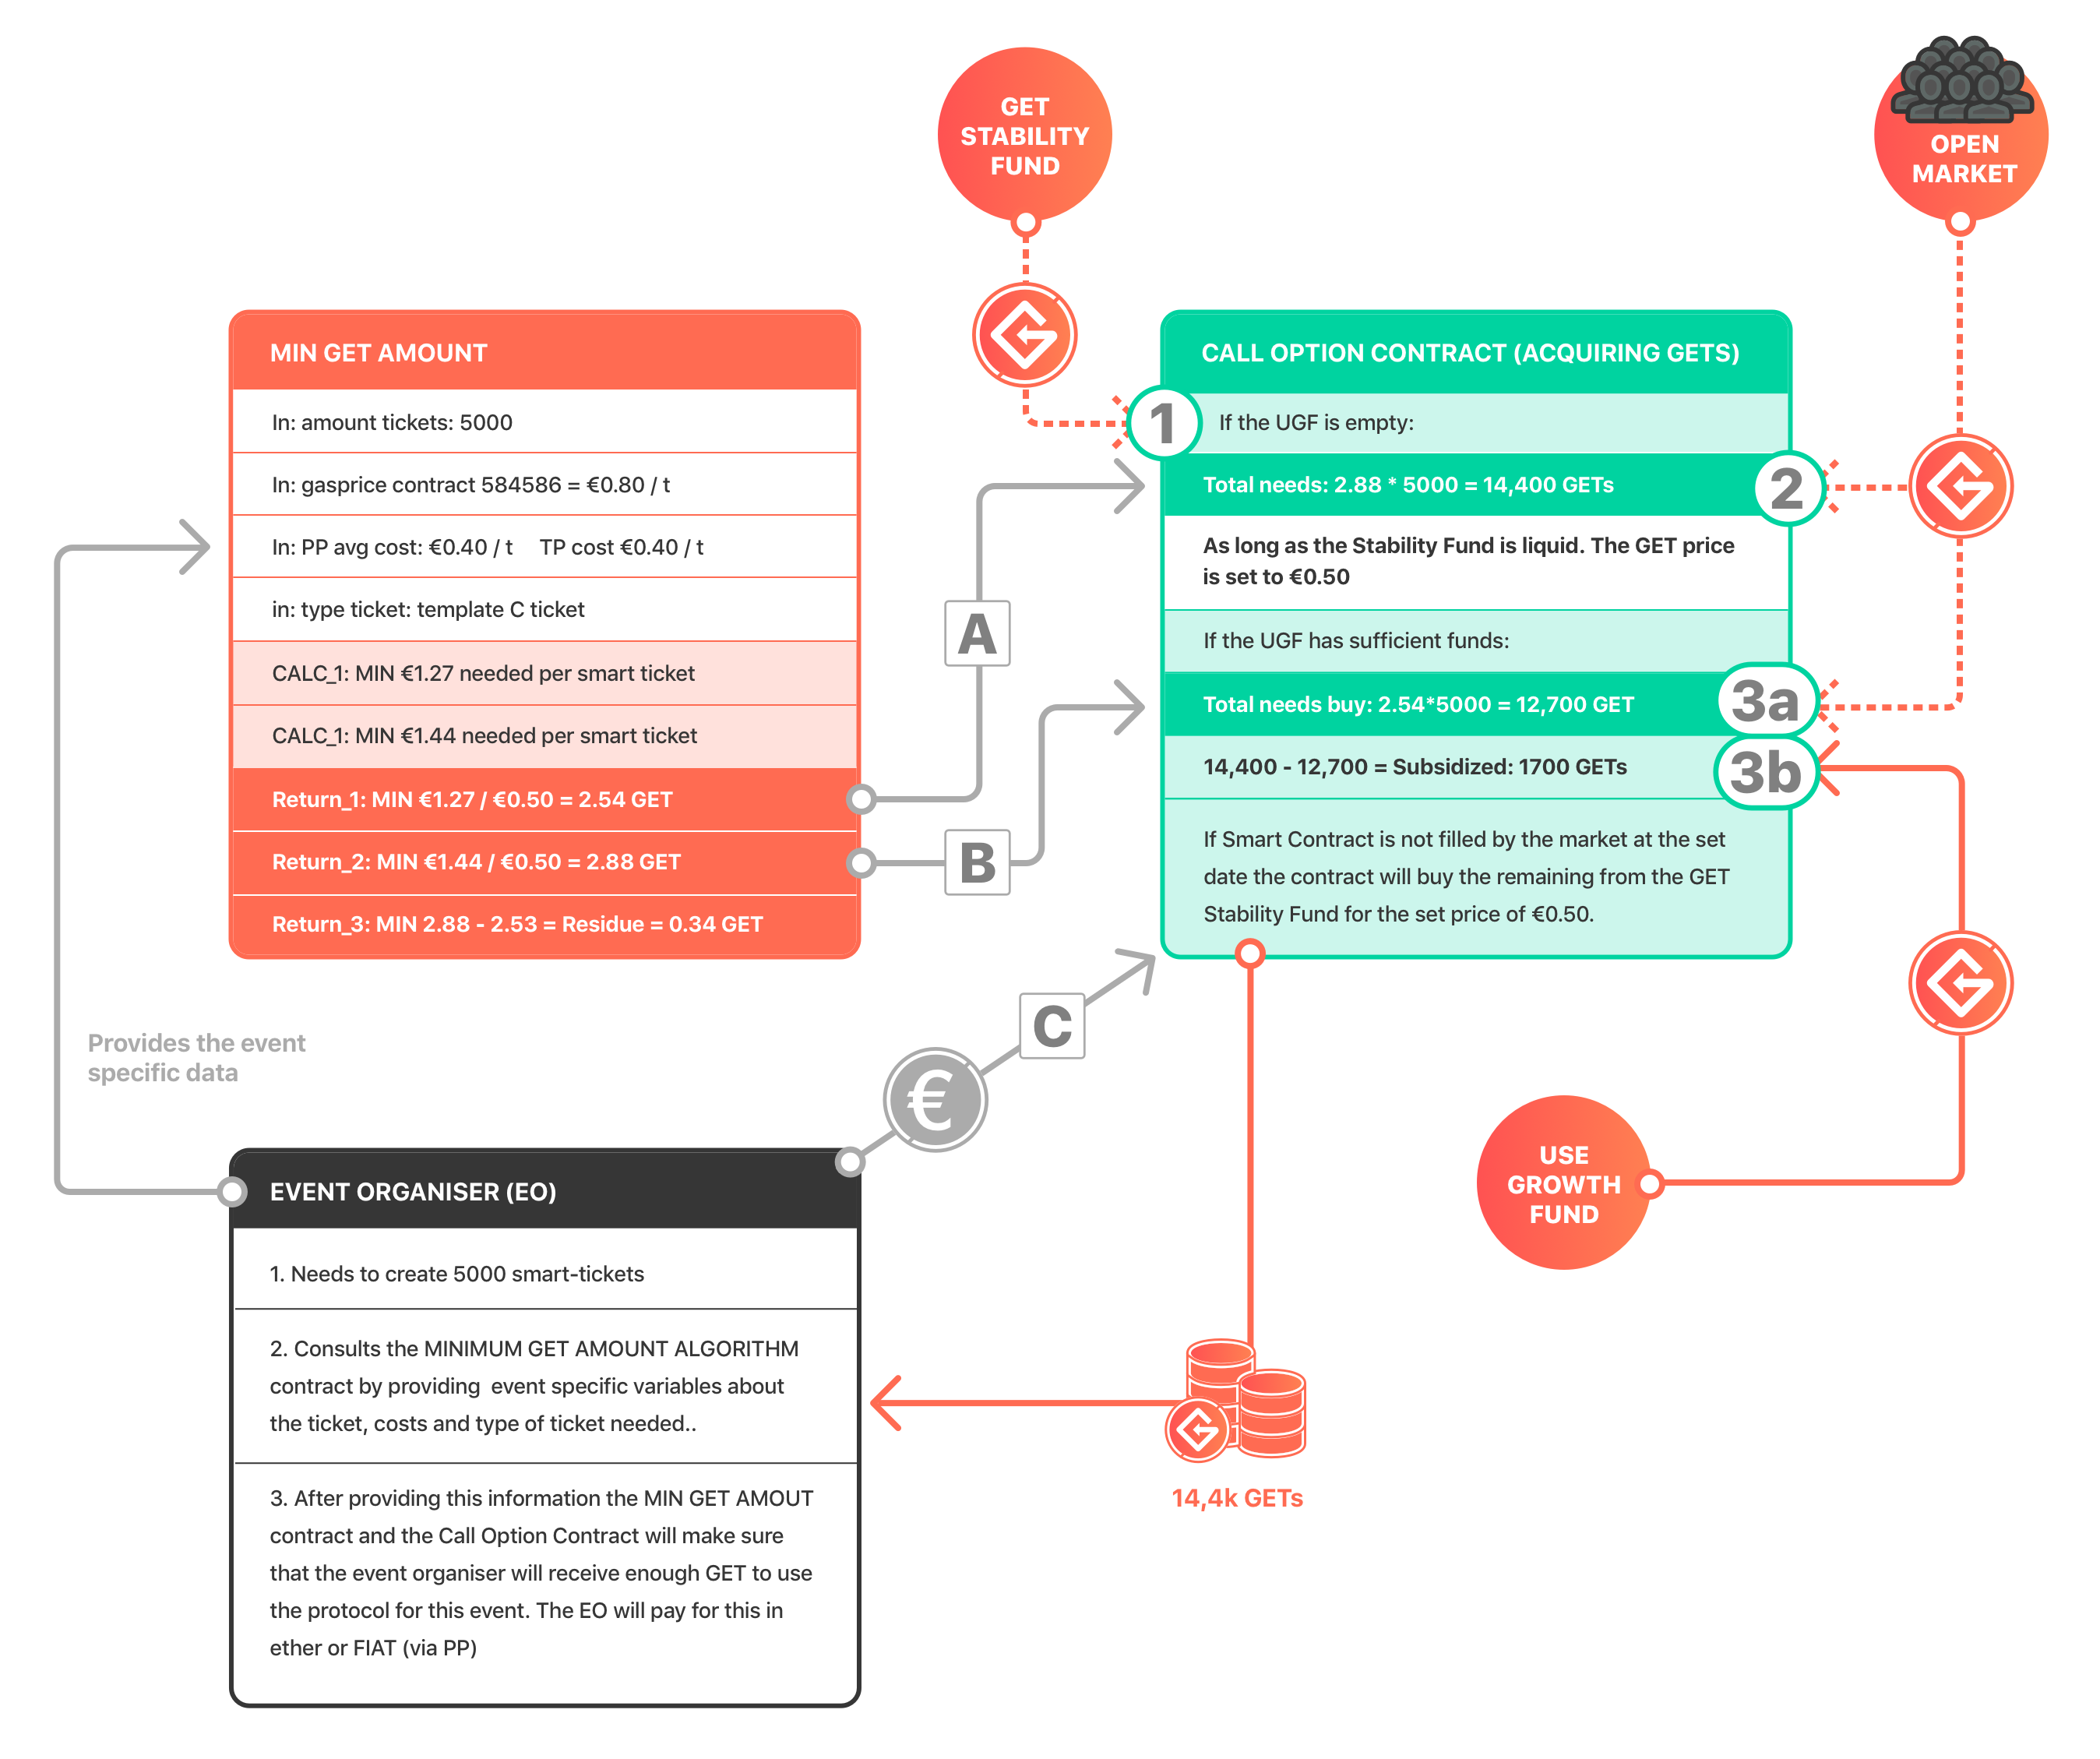
\includegraphics[width=\textwidth]{complexoption}
%     \caption{Diagram showing the GET buy-back mechanism (the GET acquisition mechanism for event organizers) The open token market will always be able to offload the GET tokens for the bottom price of \euro 0.50 if event organizers have a demand for GET. Table~\ref{complextable} displays the different steps labeled in this diagram.}
%     \label{pricingfinal}
% \end{figure}

% Please add the following required packages to your document preamble:
% \usepackage[table,xcdraw]{xcolor}
% If you use beamer only pass "xcolor=table" option, i.e. \documentclass[xcolor=table]{beamer}

% \begin{table}[h]
% \centering
% \caption{Token partitions during the crowdsale. Unsold tokens during the crowdsale will be burned.}
% \label{my-label}
% \begin{tabular}{|lcl|}
% \hline
% \rowcolor[HTML]{656565} 
% \multicolumn{1}{|l|}{\cellcolor[HTML]{656565}{\color[HTML]{FFFFFF} \textbf{Section}}} & \multicolumn{1}{l|}{\cellcolor[HTML]{656565}{\color[HTML]{FFFFFF} \textbf{Percentage}}} & {\color[HTML]{FFFFFF} \textbf{GETs}} \\ \hline
% \rowcolor[HTML]{9B9B9B} 
% \textbf{Total GET issued}                                                             & \textbf{100\%}                                                                          & \textbf{90,000k}                     \\
% \rowcolor[HTML]{EFEFEF} 
% Crowdsale                                                                             & 41\%                                                                                    & 36,900k                              \\
% Stability Fund (SF)                                                                   & 30\%                                                                                    & 27,000k                              \\
% \rowcolor[HTML]{EFEFEF} 
% User Growth Fund (UGF)                                                                & 14\%                                                                                    & 12,600k                              \\
% GUTS Team / Investors                                                                 & 13\%                                                                                    & 11,700k                              \\
% \rowcolor[HTML]{EFEFEF} 
% Promotion / Bounties                                                                  & 2\%                                                                                     & 1,800k                               \\ \hline
% \end{tabular}
% \end{table}

% The amount of GET needed is calculated by an algorithm (see page \pageref{formula_a} for more about this calculation. During the period that the initial growth fund is liquid, $ P_{res} $ costs will be subsidized. When both the stability and the growth fund are depleted, the market is assumed to be liquid and stable enough, market prices will then be used in the per-event evaluation of total transaction costs / needed value.

% Please add the following required packages to your document preamble:
% \usepackage{graphicx}
% \usepackage[table,xcdraw]{xcolor}
% If you use beamer only pass "xcolor=table" option, i.e. \documentclass[xcolor=table]{beamer}
% \begin{table}[H]
% \centering
% \resizebox{\textwidth}{!}{%
% \begin{tabular}{|lllllll}
% \hline
% \rowcolor[HTML]{343434} 
% \multicolumn{1}{|c}{\cellcolor[HTML]{343434}{\color[HTML]{FFFFFF} \textbf{1}}}                                           & \multicolumn{1}{c}{\cellcolor[HTML]{343434}{\color[HTML]{FFFFFF} \textbf{2 (UGF empty)}}}                                                                    & \multicolumn{1}{c}{\cellcolor[HTML]{343434}{\color[HTML]{FFFFFF} \textbf{3a (UGF liquid)}}}                                                                      & \multicolumn{1}{c}{\cellcolor[HTML]{343434}{\color[HTML]{FFFFFF} \textbf{3b (UGF liquid)}}}            & \multicolumn{1}{c}{\cellcolor[HTML]{343434}{\color[HTML]{FFFFFF} \textbf{A (UGF empty)}}}                                          & \multicolumn{1}{c}{\cellcolor[HTML]{343434}{\color[HTML]{FFFFFF} \textbf{B (UGF liquid)}}}                                         & \multicolumn{1}{c}{\cellcolor[HTML]{343434}{\color[HTML]{FFFFFF} \textbf{C}}}                                                                                                                           \\
% \begin{tabular}[c]{@{}l@{}}The stability fund fills\\ the remaining GET\\ requested by the buy-\\ contract.\end{tabular} & \begin{tabular}[c]{@{}l@{}}Token holders in the\\ open market send GET\\ to the buy contract and\\ receive ether for the set\\ price in return.\end{tabular} & \begin{tabular}[c]{@{}l@{}}Same as step 2.\\ Only difference being\\ that the UGF sponsors\\ the residue fraction \\ of the tokens for an \\ event.\end{tabular} & \begin{tabular}[c]{@{}l@{}}The UGF sponsors\\ the residue segment \\ of the buy contract.\end{tabular} & \begin{tabular}[c]{@{}l@{}}The min-GET-amount\\ algorithm creates a buy\\ contract for the $P_{max} $\\ of the event.\end{tabular} & \begin{tabular}[c]{@{}l@{}}The min-GET-amount\\ algorithm creates a buy\\ contract for the $P_{min} $\\ of the event.\end{tabular} & \multicolumn{1}{l|}{\begin{tabular}[c]{@{}l@{}}Event organizer pays\\ the buy contract.\\ It is possible for the\\ ticketing company to\\ provide this service for\\ the event organiser.\end{tabular}} \\ \hline
% \end{tabular}%
% }
% \caption{Take note that this table describes the situation in which the stability fund is still liquid. If the stability fund would be depleted the \euro  0.50 shown in the diagram would be replaced with the market valuation of the token.}
% \label{complextable}
% \end{table}

% Please add the following required packages to your document preamble:
% \usepackage[table,xcdraw]{xcolor}
% If you use beamer only pass "xcolor=table" option, i.e. \documentclass[xcolor=table]{beamer}

% \begin{table}[]
% \centering
% \caption{My caption}
% \label{my-label}
% \begin{tabular}{ll}
% \rowcolor[HTML]{000000} 
% \multicolumn{2}{c}{\cellcolor[HTML]{000000}{\color[HTML]{FFFFFF} \textbf{Advisory board of the GET-Protocol}}}                                                                                                                                                                                                                                     \\
% \rowcolor[HTML]{C0C0C0} 
% \multicolumn{1}{|l|}{\cellcolor[HTML]{C0C0C0}\textbf{Watse de Jong}}   & \multicolumn{1}{l|}{\cellcolor[HTML]{C0C0C0}Manager of Martin Garrix (No. 1 DJ of 2017).}                                                                                                                                                                                 \\
% \multicolumn{1}{|l|}{\textbf{Chris Payne}}                             & \multicolumn{1}{l|}{\begin{tabular}[c]{@{}l@{}}Booker at ITB Londen. Books for Adele, Maroon 5 and 100 \\ other artists in venues/events worldwide!\end{tabular}}                                                                                                         \\
% \rowcolor[HTML]{C0C0C0} 
% \multicolumn{1}{|l|}{\cellcolor[HTML]{C0C0C0}\textbf{Robert-Jan Veen}} & \multicolumn{1}{l|}{\cellcolor[HTML]{C0C0C0}\begin{tabular}[c]{@{}l@{}}Managing director Hekwerk Theater producties.Responsible\\  for 700 events selling more than 310.000 tickets per year.\\  Hekwerk is the launching customer of GUTS Tickets and GET.\end{tabular}} \\
% \multicolumn{1}{|l|}{\textbf{Arjan Poleij}}                            & \multicolumn{1}{l|}{\begin{tabular}[c]{@{}l@{}}Ticketing consultant for 15 years. Amsel Goldrace (50k attendees),\\ Guus Meeuwis (20k at.), Dutch Olymic Village \& many more!\\ Owner at Arpo Entertainment.\end{tabular}}                                               \\
% \rowcolor[HTML]{C0C0C0} 
% \multicolumn{1}{|l|}{\cellcolor[HTML]{C0C0C0}\textbf{Nyle Budlimic}}   & \multicolumn{1}{l|}{\cellcolor[HTML]{C0C0C0}Founder of Cypher Group. Experienced crypto investor and strategist.}                                                                                                                                                         \\
% \multicolumn{1}{|l|}{\textbf{Marius Jansen}}                           & \multicolumn{1}{l|}{Co-Founder of Deribit Exchange. €2 million daily turnover.}                                                                                                                                                                                           \\ \hline
% \end{tabular}
% \end{table}

% \subsection*{The protocols guaranteed exchange rate}
% As the GET token is needed in order for event organizers to sell and assign smart tickets on the GET-protocol, this will create a demand for tokens. The protocol will regulate and facilitate this GET acquisition process to ensure that event organizers can easily and cost-effectively interact with the protocol. 

% \subsection*{Budget Allocation:}
% All funds raised during the ICO will be managed by the GET Protocol foundation. This foundation will be a different legal entity as GUTS ticketing. As GUTS is a ticketing company using the GET-protocol. The foundation will control all the funds mentioned and will coordinate, finance and be responsible for the development and adoption of the GET-protocol. 


% Please add the following required packages to your document preamble:
% \usepackage[table,xcdraw]{xcolor}
% If you use beamer only pass "xcolor=table" option, i.e. \documentclass[xcolor=table]{beamer}
% \begin{table}[]
% \centering
% \caption{My caption}
% \label{my-label}
% \begin{tabular}{|llccl|}
% \hline
% \rowcolor[HTML]{343434} 
% {\color[HTML]{FFFFFF} \textbf{Stage}}                                     & {\color[HTML]{FFFFFF} \textbf{Price / GET}} & \multicolumn{1}{l}{\cellcolor[HTML]{343434}{\color[HTML]{FFFFFF} \textbf{GET / Ether}}} & \multicolumn{1}{l}{\cellcolor[HTML]{343434}{\color[HTML]{FFFFFF} \textbf{Percentage of crowdsale}}}                & {\color[HTML]{FFFFFF} \textbf{GET in Tier}}                \\
% \textbf{Tier 1}                                                           & \euro 0.42                                  & 236.26                                                                                  & 20\%                                                                                                               & 7,380k                                                     \\
% \rowcolor[HTML]{EFEFEF} 
% \textbf{Tier 2}                                                           & \euro 0.44                                  & 607.23                                                                                  & 20\%                                                                                                               & 7,380k                                                     \\
% \textbf{Tier 3}                                                           & \euro 0.47                                  & 568.57                                                                                  & 20\%                                                                                                               & 7,380k                                                     \\
% \rowcolor[HTML]{EFEFEF} 
% \textbf{Tier 4}                                                           & \euro 0.49                                  & 545.36                                                                                  & 20\%                                                                                                               & 7,380k                                                     \\ \hline
% \begin{tabular}[c]{@{}l@{}}Buy-back price\\ by GET-protocol*\end{tabular} & \euro 0.50                                  & \multicolumn{1}{c|}{534.46**}                                                           & \multicolumn{2}{l|}{\begin{tabular}[c]{@{}l@{}}* See whitepaper p. 18 for buy back details.\\ ** This is dependent on the ethereum price at \\ the buy back time.\end{tabular}} \\ \hline
% \end{tabular}
% \end{table}


% \begin{figure}[H]
% \centering
% 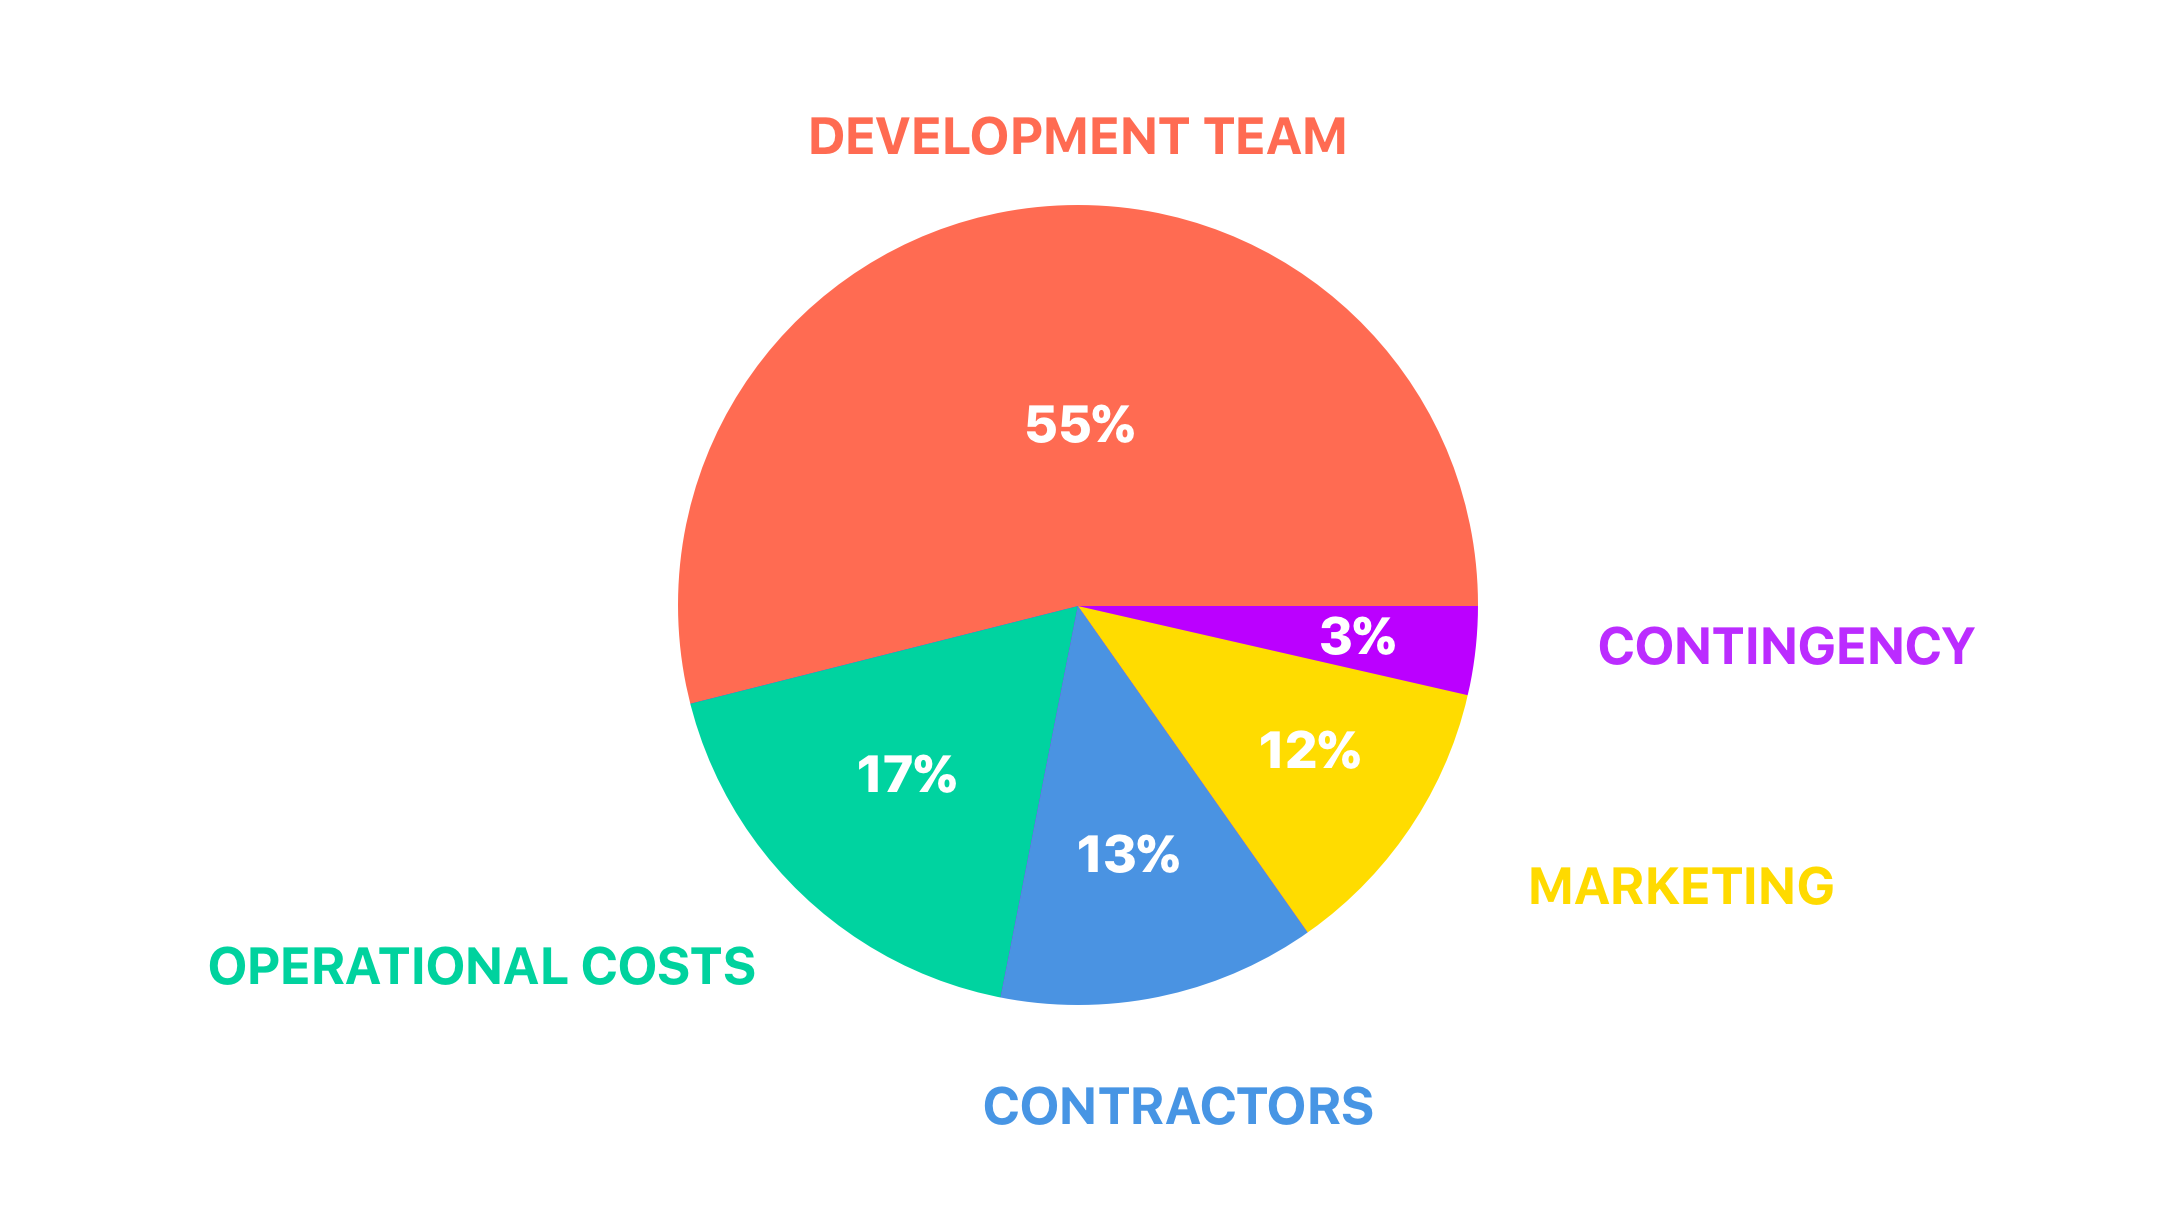
\includegraphics[width=.5\textwidth]{4}
% \caption{Pie chart displaying the budget allocation of the funds raised in the ICO.}
% \end{figure}


% Please add the following required packages to your document preamble:
% \usepackage[table,xcdraw]{xcolor}
% If you use beamer only pass "xcolor=table" option, i.e. \documentclass[xcolor=table]{beamer}
% \begin{table}
% \centering
% % \caption{My caption}
% % \label{team_table}
% \begin{tabular}{l}
% \hline
% \rowcolor[HTML]{000000} 
% {\color[HTML]{FFFFFF} \textbf{The Team}} \\ \hline
% \rowcolor[HTML]{C0C0C0} 
% - CEO | Maarten Bloemers  \faLinkedin                                              \\ \hline
% - CCO | Tom Roetgering                                                 \\ \hline
% \rowcolor[HTML]{C0C0C0} 
% - CTO | Ivo van der Wijk                                                \\ \hline
% UX/Developer | Frans Twisk                                              \\ \hline
% \rowcolor[HTML]{C0C0C0} 
% Developer | Stavros Champilomatis                                       \\ \hline
% Developer | Kasper Keunen                                               \\ \hline
% \rowcolor[HTML]{C0C0C0} 
% Developer | Mark Arts                                                   \\ \hline
% Marketing | Sander Regtuijt                                             \\ \hline
% \rowcolor[HTML]{C0C0C0} 
% Operations | Denise van der Meulen                                      \\ \hline
% \multicolumn{1}{|c|}{You? GUTS Tickets is hiring!}                      \\ \hline
% \end{tabular}
% \end{table}

% \begin{table}
% \centering
% % \caption{My caption}
% % \label{my-label}
% \begin{tabular}{r}
% \rowcolor[HTML]{000000} 
% \multicolumn{2}{c}{\cellcolor[HTML]{000000}{\color[HTML]{FFFFFF} \textbf{Advisory board of the GET-Protocol}}}                                                                                                                                                                                                                                     \\
% \rowcolor[HTML]{C0C0C0} 
% \multicolumn{1}{|l|}{\cellcolor[HTML]{C0C0C0}\textbf{Watse de Jong}}   & \multicolumn{1}{l|}{\cellcolor[HTML]{C0C0C0}Manager of Martin Garrix (No. 1 DJ of 2017).}                                                                                                                                                                                 \\
% \multicolumn{1}{|l|}{\textbf{Chris Payne}}                             & \multicolumn{1}{l|}{\begin{tabular}[c]{@{}l@{}}Booker at ITB Londen. Books for Adele, Maroon 5 and 100 \\ other artists in venues/events worldwide!\end{tabular}}                                                                                                         \\
% \rowcolor[HTML]{C0C0C0} 
% \multicolumn{1}{|l|}{\cellcolor[HTML]{C0C0C0}\textbf{Robert-Jan Veen}} & \multicolumn{1}{l|}{\cellcolor[HTML]{C0C0C0}\begin{tabular}[c]{@{}l@{}}Managing director Hekwerk Theater producties.Responsible\\  for 700 events selling more than 310.000 tickets per year.\\  Hekwerk is the launching customer of GUTS Tickets and GET.\end{tabular}} \\
% \multicolumn{1}{|l|}{\textbf{Arjan Poleij}}                            & \multicolumn{1}{l|}{\begin{tabular}[c]{@{}l@{}}Ticketing consultant for 15 years. Amsel Goldrace (50k attendees),\\ Guus Meeuwis (20k at.), Dutch Olymic Village \& many more!\\ Owner at Arpo Entertainment.\end{tabular}}                                               \\
% \rowcolor[HTML]{C0C0C0} 
% \multicolumn{1}{|l|}{\cellcolor[HTML]{C0C0C0}\textbf{Nyle Budlimic}}   & \multicolumn{1}{l|}{\cellcolor[HTML]{C0C0C0}Founder of Cypher Group. Experienced crypto investor and strategist.}                                                                                                                                                         \\
% \multicolumn{1}{|l|}{\textbf{Marius Jansen}}                           & \multicolumn{1}{l|}{Co-Founder of Deribit Exchange. €2 million daily turnover.}                                                                                                                                                                                           \\ \hline
% \end{tabular}
% \end{table}

% GET Foundation: GUTS Tickets came to the conclusion that to truly unleash a revolution in the ticketing industry, the technology it developed should be further developed and operated from within a separate foundation so other ticketing companies will be able to make use of the GET-protocol . Moreover, GUTS Tickets realised that in order to increase the pace and expand scope, such a foundation would require sufficient resources. 

% This is why a separate foundation fully dedicated to designing the GET-Protocol has been incorporated: de Stichting GET Protocol Foundation (the GET Foundation, trade registry number 69771138) a foundation incorporated in and under the laws of the Netherlands. A Foundation under Dutch law has a board, and does not have shareholders or members. It may operate a business, employ persons, own assets and enter into agreements. Importantly, however, a foundation under Dutch law may not distribute profits.

% The way forward: GUTS Tickets developed and tested what we will here coin the "genesis" version to the GET-Protocol, which will be further developed and tested by the GET Foundation. As we will explain in further chapters, GUTS Tickets will transfer the requisite assets to the GET Foundation and will serve as launching customer of the GET-Protocol. As the GET-Protocol moves to a fully distributed smart event ecosystem, we intend that other event organizers and ticketing companies can use our open source infrastructure to develop their own use case for the GET-Protocol. We want the GET-Protocol and the tools associated with it to become the standard for smart event ticketing. After years of being ripped off and defrauded, festival and theatre visitors deserve a secure, fair and well-engineered event protocol.
\vspace{-0.3cm}

% \textcolor{gutsoranje}{the complete whitepaper}
\begin{center}
	Want to know more about GUTS Tickets or the GET Protocol? \\ 
    Visit our \href{https://guts.tickets/}{\textcolor{gutsoranje}{website}} or check out \href{https://guts.tickets/files/GET-Whitepaper-GUTS-Tickets-latest.pdf}{ \textcolor{gutsoranje}{the complete whitepaper!}}
\end{center}

% \href{https://guts.tickets/files/GET-Whitepaper-GUTS-Tickets-latest.pdf}{the complete whitepaper}
\end{document}
